\section*{Introdução}
\addcontentsline{toc}{section}{Introdução}
\label{sec:intro}

Com os recentes avanços das tecnologias, especificamente nas últimas décadas e devido a democratização da Internet, nossa sociedade tem caminhado para um cenário cada vez mais conectado. Se antes apenas super-computadores e máquinas robustas eram conectadas à rede, a tendência nos próximos anos é que dispositivos cada vez menores também tenham seu espaço na Internet.
A essa tendência chamamos \textit{Internet of Things} ( Internet das Coisas ou IoT). É uma nova visão que descreve objetos fazendo parte da rede, onde cada um deles é unicamente identificado, acessível através da rede, com posição e estado conhecido, captando informações sensoriais ou agindo sobre o ambiente. Serviços são construídos com base nesses objetos \cite{ComputerWorld}. Estima-se que até 2020, sejam investidos cerca de US\$ 267 bi na indústria e serviços voltados para IoT \cite{BCGPerspectives,Forbes}, ver Figura~\ref{fig:iotstack}.

\begin{figure}[h!]
	\begin{center}
		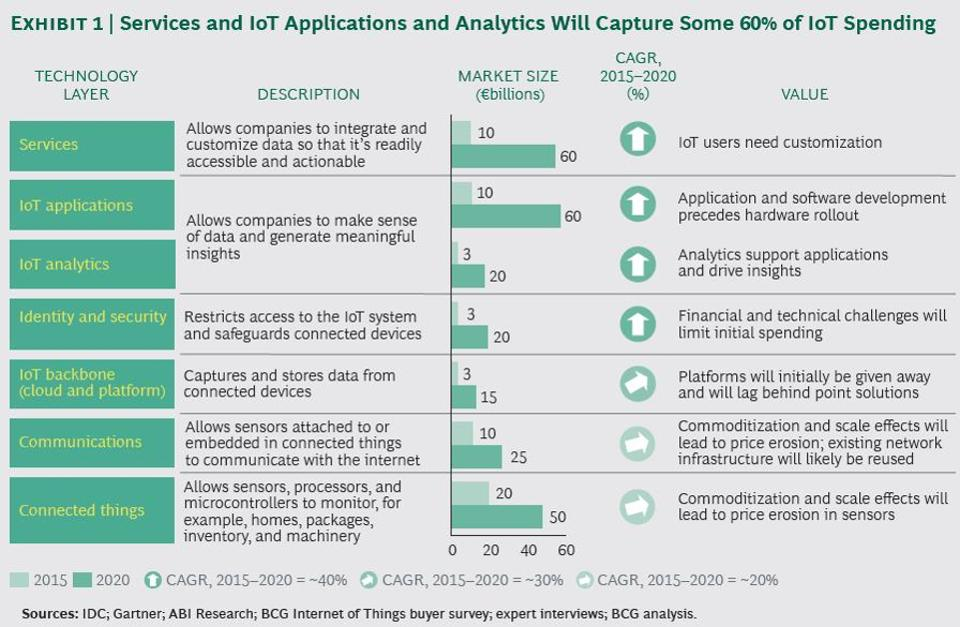
\includegraphics[width=1.085\textwidth]{./img/IoT-Stack}
		\caption{Dados dos investimentos futuros a \textit{IoT}.}
		\label{fig:iotstack}
	\end{center}
\end{figure}

As pressões comerciais são implacáveis. Como resultado disso, os requisitos estão se tornando cada vez mais complexos, exigindo assim uma maior conectividade entre dispositivos legados e novos, o que leva à necessidade de personalizações. À medida que a conectividade aumenta, novos pontos de ataque surgem, levando as empresas a ficarem cada vez mais preocupadas com percas provenientes de ataques cibernéticos. Devido a isso, as empresas enfrentam um desafio ao encontrar uma solução que atenda as suas necessidades específicas, e isso está impulsionando a necessidade de dispositivos IoT personalizados. Assim surgem os Smart IoT Gateway \cite{EETAsia}. 

Para entender melhor como as tecnologias envolvidas funcionam, o objetivo deste trabalho é construir um Smart IoT Gateway open-source, funcional e de uso simples, onde usuários cadastrem ações baseados nos dados enviados por um sensor cadastrado. Neste trabalho não temos como objetivo construir um projeto de hardware para um Gateway IoT.
